\documentclass{standalone}
\usepackage{tikz}
\usepackage{pgfplots}
% \pgfplotsset{colormap={b}{gray(0cm)=(0); gray(1cm)=(0.8)}}
% all other packages and stuff you need for the picture
%
\begin{document}
{
\centering
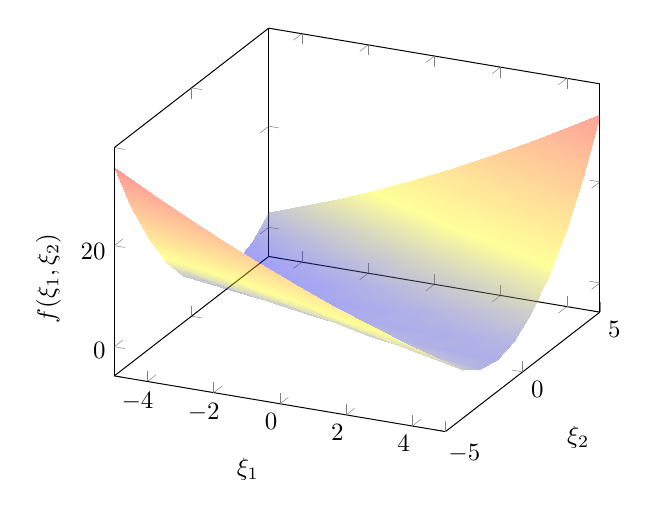
\begin{tikzpicture}[xscale=0.9,yscale=0.9]
    \begin{axis}[
        samples=10,
        % colormap name=b,
        xlabel={$\xi_1$},
        ylabel={$\xi_2$},
        zlabel={$f(\xi_1,\xi_2)$},
        ],
        \addplot3 [surf,shader=interp,opacity=0.4] {0.0481 + 0.1330*x - 0.3547*y + 0.0867*(x^2) + 0.7117*(y^2) + 0.5805*x*y};
    \end{axis}[]
\end{tikzpicture} \hspace{2cm}
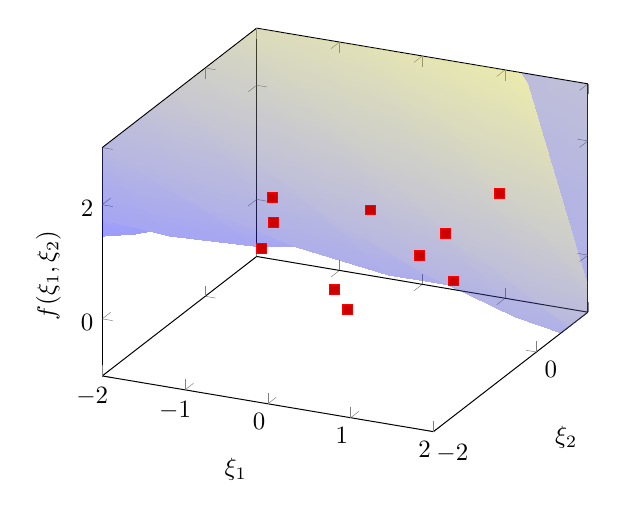
\begin{tikzpicture}[xscale=0.9,yscale=0.9]
    \begin{axis}[
        samples=10,
        % colormap name=b,
        xlabel={$\xi_1$},
        ylabel={$\xi_2$},
        zlabel={$f(\xi_1,\xi_2)$},zmax=3,zmin=-1,ymax=1,ymin=-2,xmin=-2,xmax=2,
        ],
        \addplot3 [surf,shader=interp,opacity=0.4] {0.0481 + 0.1330*x - 0.3547*y + 0.0867*(x^2) + 0.7117*(y^2) + 0.5805*x*y};
        \addplot3+[only marks] coordinates{
                 (0,0,1)(1,0,0)(1.0675,0.7756,1)
                (0.3090,0.9511,0)(-0.4078,1.2549,1)
               (-0.8090,0.5878,-1)(-1.3195,0,0)
               (-0.8090,-0.5878,1)(-0.4078,-1.2549,2)
                (0.3090,-0.9511,0)(1.0675,-0.7756,1)}
        ;
    \end{axis}[]
\end{tikzpicture}
}
\end{document}